\subsection{Satisfiability and Satisfiability Modulo Theories}

The satisfiability problem consists of finding a 
propositional assignment for a propositional formula. 
This problem is at the core level of complexity theory, 
defining an important class of problems known as 
NP, which includes problems whose
algorithms seem to be intractable.
Developments in algorithms and heuristics 
\cite{10.5555/2898950, 
935565} have made it possible to use satisfiability 
algorithms 
to solve real-world problems in 
verification \footnote{These
  advances do not provide an answer to the well-known P vs. NP
  problem. There are results indicating a class of problem instances
  for many of the SAT algorithms which cannot be solved in less that
  \bigO{2^n} steps \cite{10.5555/2898950}.
}.

The DPLL algorithm \cite{10.1145/368273.368557} 
(and other extensions) is the algorithm
found in many SAT solvers. Fundamentally, it is a search-based algorithm
which implements operators (decide, unit-propagation, backtrack)
to find a satisfiable assignment. If the algorithm is not able to
find a satisfying assignment for a formula, then it is possible to 
extract a \emph{resolution proof} based on the traces of the search
operations.

%\begin{example}

  \begin{figure}
    \centering
    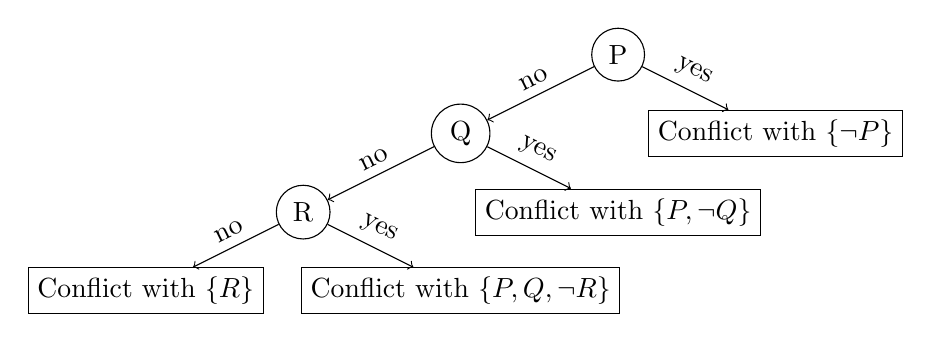
\begin{tikzpicture}[->]
      \node(p) at (6, 5) [circle, draw] {P};
      \node(q) at (4,4) [circle, draw] {Q};
      \node(r) at (2, 3) [circle, draw] {R};
      \node(expl1) at (8, 4) [rectangle, draw] {Conflict with $\{\neg P\}$};
      \node(expl2) at (6, 3) [rectangle, draw] {Conflict with $\{P, \neg Q\}$};
      \node(expl3) at (4, 2) [rectangle, draw] {Conflict with $\{P, Q, \neg R\}$};
      \node(expl4) at (0, 2) [rectangle, draw] {Conflict with $\{R\}$};

      \path[every node/.style={sloped,anchor=south,auto=false}]
      (p) edge node {yes} (expl1)   
      (p) edge node {no}  (q)   
      (q) edge node {yes} (expl2)
      (q) edge node {no}  (r)
      (r) edge node {yes} (expl3)
      (r) edge node {no}  (expl4);
    \end{tikzpicture}

    \caption{Example of DPLL execution on 
      $\{\{\neg P\}, \{P, Q, \neg R\}, \{R\}, 
    \{P, \neg Q\} \}$} \label{dpll_figure}

  \end{figure}

  %We can see that the following resolution proof resembles the
  %structure of the DPLL execution on figure \ref{dpll_figure}, i.e.
  %if we rotate the proof-tree and mark the nodes by the pivots used
  %we obtained a similar tree obtained by the execution of the DPLL
  %algorithm. This fact becomes relevant because it enables us 
  %to construct a resolution proof from the traces of a SAT 
  %solver used
  %in the theory combination part of the implementation. 

  %\begin{figure}
    %\centering
    %\begin{prooftree}
      %\hypo[]{\neg P}
      %\hypo[]{P \lor Q \lor \neg R}
      %\infer2[$res_P$]{Q \lor \neg R}
      %\hypo[]{R}
      %\infer2[$res_R$]{Q}
      %\hypo[]{P \lor \neg Q}
      %\infer2[$res_Q$]{P}
      %\hypo[]{\neg P}
      %\infer2[$res_P$]{\bot}
    %\end{prooftree}
    %\caption{Example of resolution proof} 
    %\label{example_resolution_proof}
  %\end{figure}

%\end{example}

We can extend this approach to work not only with propositional
variables but with terms of more complex signatures 
\cite{10.5555/1391237}. If we are given a boolean combination 
of formulas from any theory that is capable of deciding the 
satisfiability of any conjunction of formulas in the theory, 
by using a \emph{lazy framework} integration with a SAT solver it is 
possible to find either a model or declare unsatisfiable such boolean
combination as follows: (i) first abstract the literals in the boolean
combination to (pseudo) boolean propositions; (ii) find a satisfying
assignment (using a SAT solver) of the (pseudo) boolean propositions;
(iii) using the theory solver, test if the collection of positive
and negative literals induced by the pseudo boolean variables is
satisfiable; (iv) if it is then declare the formula satisfiable, 
otherwise \emph{learn} (or block) the pseudo boolean clause obtained
(by negating the conjunction of boolean constraints) in the SAT
solver and repeat from step (ii); (v) if it is not possible to
find a satisfying assignment for the pseudo boolean variables, 
declare the original formula to be unsatisfiable.

These algorithms are used in the last section of the thesis work.
The implementation for the interpolation combination method
in \cite{10.1007/11532231_26} requires a resolution-based
proof in order to compute partial interpolants by integrating
Pudlak's algorithm.

%%% Local Variables:
%%% mode: latex
%%% TeX-master: "main"
%%% End:
